\documentclass[11pt, a4paper]{article}
\usepackage[utf8]{inputenc}
\usepackage{graphicx}
\usepackage{amsmath}
\usepackage{hyperref}
\usepackage{booktabs}
\usepackage{enumitem}
\usepackage{geometry}
\geometry{margin=2.5cm}

\title{Sketch-Based 3D Shape Generation\\
\large Visual Computing Mini Project}
\author{Your Name}
\date{\today}

\begin{document}

\maketitle

\begin{abstract}
This report documents the design, implementation, and evaluation of a sketch-based 3D modeling system that couples human-friendly 2D input with procedural geometry generators. The prototype combines an SVG-capable browser editor, Potrace-assisted raster vectorisation, OpenCV-based mask processing, a trio of custom C++ geometry modules, a lightweight software renderer, and a React/Three.js frontend. Users can draw or upload sketches, the backend extracts contours, profiles, and scalar fields, and three modeling modes (extrusion, revolution, and height-map inflation with optional distance-field ``bulge'') convert these signals into meshes that can be viewed interactively. We describe the implemented algorithms, the client--server architecture, the parameterization exposed at the user interface, and a mixed qualitative and quantitative evaluation that covers visual fidelity, runtime behaviour, and usability. The system demonstrates an end-to-end workflow from sketch acquisition to mesh visualization within the constraints of the visual computing mini-project.
\end{abstract}

\section{Introduction}
Three-dimensional modeling is traditionally associated with complex software and a steep learning curve. Novice users often struggle with professional CAD tools, and even experts may find them cumbersome during early ideation. Sketch-based modeling offers an alternative interaction style: instead of manipulating vertices or solids directly, users draw silhouettes or profiles on a two-dimensional canvas and expect the system to infer a plausible three-dimensional interpretation~\cite{igarashi2023teddy}. Classic systems such as Teddy demonstrated how freehand sketches can be inflated into volumetric shapes, while follow-up work explored contour vectorization, simplification, and topology preservation for sketch vectorization~\cite{shade1998layered,scharstein2002taxonomy}. Modern deployments often combine OpenCV-style processing on the backend with WebGL viewers on the frontend, underscoring the tight coupling between perception and rendering in visual computing.

Turning casual sketches into reliable geometry is not straightforward. Strokes can be noisy, incomplete, or ambiguous, and the resulting models must remain stable while parameters are edited in real time. The goal of this project is therefore to build an end-to-end system that accepts 2D sketches, processes them with computer vision techniques, and generates 3D meshes fast enough to support interactive use. The system targets three modeling modes: extrusion, revolution, and height-map inflation. Together they cover common shape families ranging from mechanical parts with sharp edges, through rotational pottery forms, to soft organic domes.

In the remainder of this document we describe the pipeline architecture, highlight the most relevant implementation details on both the backend and the frontend, and outline the qualitative and quantitative evaluation protocol that demonstrates the system's behaviour under realistic sketching scenarios.

\section{System Architecture}
\subsection{System Overview}
Figure~\ref{fig:pipeline} summarizes the implemented pipeline. The frontend is a React application that offers a drawing canvas and parameter controls. The canvas supports both a freehand brush and a small set of geometric primitives such as rectangles, circles and straight lines, which can be placed by dragging in a way that resembles simple shape tools in presentation software, and the toolbar also provides an undo button and a line-width slider so users can tune stroke thickness before committing a sketch. When the user uploads or saves a sketch, the image is sent as a base64-encoded PNG to the C++ backend via a REST endpoint. The backend stores the image on disk and invokes the \texttt{SketchProcessor}, which converts the raster into a compact representation consisting of a planar contour, a radial profile and a height map. This sketch data is routed through the \texttt{PipelineController} to one of three geometry generators (extrusion, revolution or height-map). The resulting mesh is passed both to a CPU-based \texttt{OffscreenRenderer}, which produces a bitmap preview, and to a \texttt{MeshSerializer}, which writes vertex positions, normals and triangle indices to a JSON file. The frontend periodically queries a ``latest result'' endpoint, loads the JSON mesh into a Three.js viewer for interactive inspection, and displays the software-rendered bitmap alongside it.

\begin{figure}[t]
    \centering
    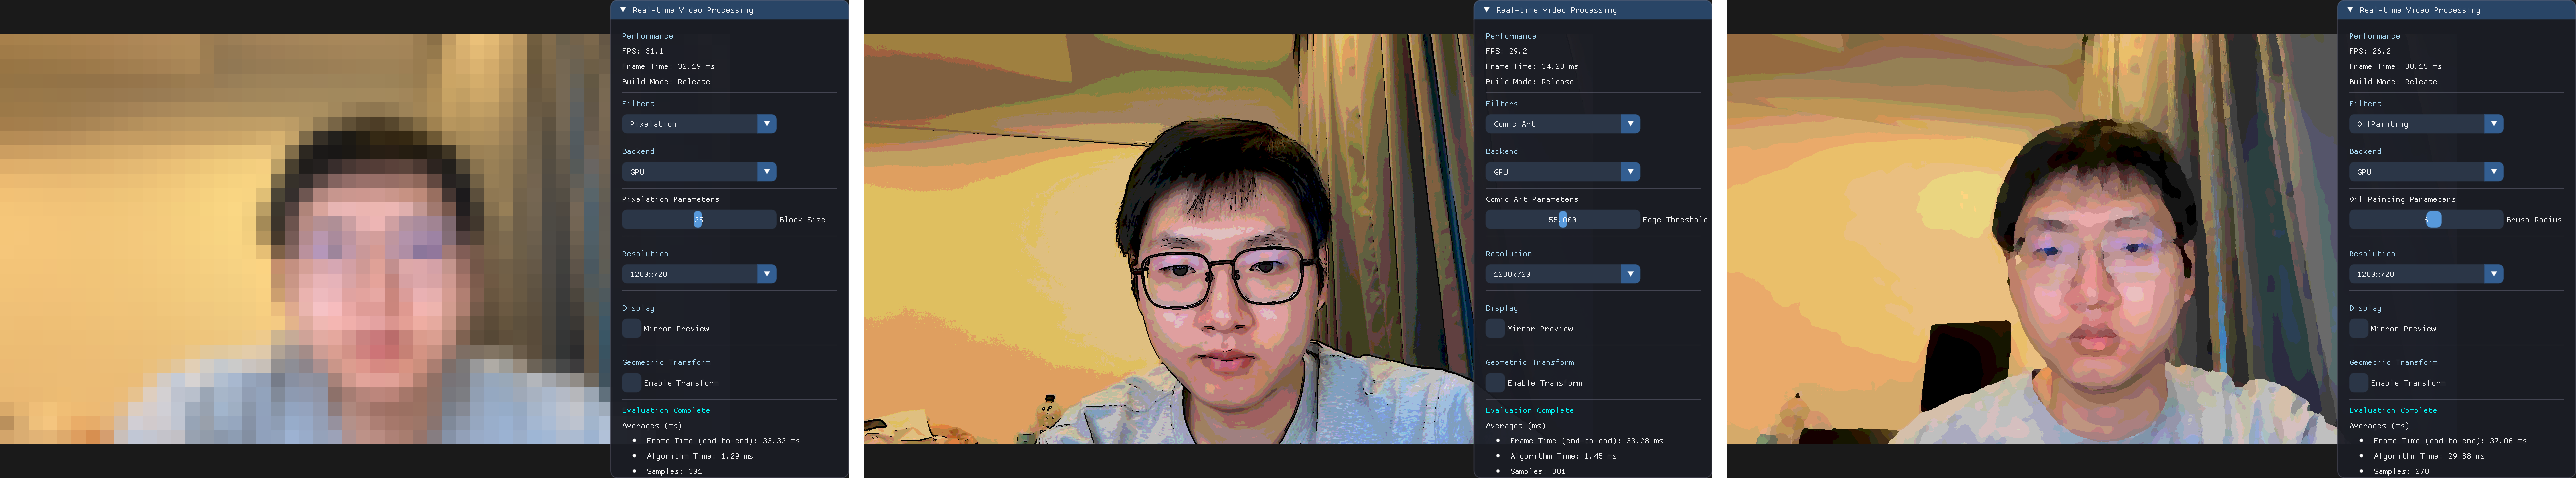
\includegraphics[width=0.85\linewidth]{Figures/overviewfilter.png}
    \caption{System overview. The React frontend sends sketches to a C++ backend, which processes them with OpenCV, generates geometry in three modes, and returns both a software-rendered image and a JSON mesh that is visualized with Three.js.}
    \label{fig:pipeline}
\end{figure}

\subsection{Sketch Processing}
The frontend no longer sends raster screenshots of the drawing canvas. Instead, sketches are exported as SVG files that contain a small metadata block (\texttt{<metadata id="sketch-data">}) with a JSON description of every stroke, rectangle, ellipse and straight line, all normalized to the $576\times640$ drawing space. Each entry lists the sampled polyline points, whether the shape is closed, and the intended stroke width. This makes the transfer format lossless and avoids the ambiguity caused by anti-aliasing or image compression.

On the backend we first inspect the uploaded filename. If it is an SVG, we parse the metadata with \texttt{nlohmann::json}, convert every polyline into a list of \texttt{cv::Point}s and rasterize it directly into an OpenCV mask using \texttt{fillPoly} and \texttt{polylines}. The rasterization honours the per-shape stroke widths so that open polylines retain their apparent thickness. If the upload is a legacy bitmap (for example when users import an existing PNG), we still apply a lightweight CLAHE-enhanced threshold, but rather than rolling our own contour extraction we now convert the binarised mask into PBM format and invoke Potrace~1.16. Potrace is a battle-tested vectorisation tool that recovers clean polylines from noisy black-and-white sketches, so it preserves multiple parallel strokes and sharp corners much better than heuristics built on top of \texttt{findContours}. The resulting SVG paths are fed back into the same metadata/parser, which keeps the remainder of the pipeline unchanged while dramatically improving robustness on scanned drawings.

Regardless of origin, the resulting binary mask is optionally dilated by the global stroke-thickness parameter, processed with adaptive open/close filters and finally closed with a fixed $5\times5$ kernel to bridge small gaps. We then extract every connected component via \texttt{findContours}. Components smaller than $5\%$ of the largest contour are treated as noise; the rest are simplified with \texttt{approxPolyDP}, normalized to $[-0.5,0.5]^2$, and stored in a list that now supports arbitrary numbers of disjoint loops. The dominant loop is still cached separately for backward compatibility with parts of the pipeline that expect a single contour, but extrusion and height-map modules consume the full set of loops directly.

To obtain a stable polygonal contour we draw each component into its own mask before simplification, guaranteeing that open strokes are sealed and converted into solid regions. Revolution profiles and height maps reuse the filled mask as before: 64 scanlines sample the radial profile around the vertical axis, and the mask is downsampled to a $64\times64$ scalar field for the height-map generator.

For the revolution profile we reuse the filled mask. The processor samples 64 horizontal scanlines across the image. On each scanline it measures the maximum distance from the vertical image center to a foreground pixel; this distance becomes a radial coordinate, while the scanline position is mapped to a normalized height. The resulting sequence of radius--height pairs forms the one-dimensional profile used by the revolution module. If the mask does not contain any foreground pixels, a small default profile is substituted so that the rest of the pipeline continues to function.

Height-map input is derived from the same filled mask. The mask is resized to a fixed $64 \times 64$ grid with area resampling, and each pixel value is normalized to the range $[0, 1]$. These samples are flattened into a vector that serves as the base scalar field for the height-map generator. When OpenCV is not available, the processor falls back to a synthetic square contour and a Gaussian bump height map to keep the system operational.

\subsection{Geometry Generation}
\subsubsection{Extrusion}
The extrusion module interprets the planar contour as a closed polygon in the $xy$ plane and produces a solid by duplicating it at two $z$ offsets. Before meshing, each contour loop can be smoothed by a configurable number of midpoint subdivision steps, which recursively insert midpoints on every edge and thereby increase sampling density while softening sharp corners. The effective loops, already influenced by the stroke-thickness dilation in the image space, are used for all subsequent computations. If multiple disjoint loops are present (e.g., letters with holes or separate parts), the generator extrudes each loop independently and merges the resulting meshes by offsetting vertex indices, yielding a single combined mesh without forcing users to draw only one silhouette.

Vertices for the bottom and top caps are placed at $z=-d/2$ and $z=+d/2$, where $d$ is the user-controlled extrusion depth. Both caps use the same polygon in the current implementation, so the footprint of the shape is constant along the extrusion direction. Caps are triangulated with a simple ear-clipping algorithm that enforces consistent counter-clockwise winding and rejects non-convex ears that would overlap existing triangles.

Side walls are constructed by connecting corresponding vertices on the bottom and top rings. For each edge of the contour we create a quad between the two layers and split it into two triangles. Edge directions are used to compute outward-facing normals by taking the perpendicular vector in the plane and normalizing it, so that shading on the side walls reflects the original silhouette.

\subsubsection{Revolution}
The revolution module takes the radial profile produced by the sketch processor and sweeps it around a vertical axis to create a surface of revolution. The profile is sampled at a user-specified number of angular segments. For each segment we compute cosine and sine values for the current angle and rotate every profile point into three-dimensional space. The $x$ coordinate of the revolution axis is configurable; a non-zero offset yields rings that do not pass through the origin, which is useful for donut-like shapes.

The implementation supports both solid and hollow tubes. In solid mode, one vertex is generated per profile point and segment. In hollow mode, two vertices are created: an outer vertex at radius $r$ and an inner vertex at radius $r - t$, where $t$ is the wall thickness parameter clamped to non-negative values. Outer vertices use outward-pointing normals derived from the rotation angle; inner vertices use inverted normals so that lighting on the inner wall is correct.

Quad strips are formed between adjacent angular segments and between neighbouring profile samples. These strips are split into triangles and written into the index buffer. When end caps are enabled, additional vertices are inserted on the top and bottom center points along the revolution axis, and triangle fans connect these centers to the first and last rings of the profile, sealing the model.

\subsubsection{Height Map}
The height-map generator interprets the scalar field from the sketch processor as samples on a regular grid. An optional blur stage applies a separable box filter whose effective radius is proportional to a user-controlled blur parameter. This operation smooths the field and attenuates small-scale noise. The blurred samples are then scaled by a global height factor when converted into vertex elevations. To better match users' expectations for ``inflated'' sketches, we additionally compute a distance transform over the binary silhouette and blend it with the raw mask according to a ``bulge strength'' parameter. Setting the slider to zero preserves the hard, plateau-like height field, whereas higher values progressively replace it with a normalized distance dome, producing the rounded ``baozi'' effect without requiring painters to supply grayscale artwork.

If the user chooses to keep the base plane, the generator builds a full grid mesh. Each grid point becomes a vertex whose $x$ and $z$ coordinates span the interval $[-0.5, 0.5]$, and whose $y$ coordinate equals the scaled height sample. Neighbouring grid cells are triangulated in a regular pattern to yield a height-field surface. If the base plane is disabled, the generator instead iterates over grid cells and emits geometry only for cells whose four corner samples exceed a small threshold, producing isolated patches that roughly follow the drawn strokes while leaving the background empty.

\subsection{Rendering and Interaction}
The backend renderer is a self-contained software rasterizer implemented in C++. It constructs a camera using a simple look-at matrix and a perspective projection, transforms all mesh vertices into clip space and then into screen space, and rasterizes each triangle into a color and depth buffer using barycentric coordinates. Lighting is a single directional light with a constant ambient term, and colors are written into an RGB bitmap. The bitmap is stored as a 24-bit BMP file on disk and later served to the frontend as a static asset.

Interactive inspection happens entirely in the browser. The React frontend uses \texttt{@react-three/fiber} and \texttt{@react-three/drei} to create a Three.js scene with an orbit controller, a ground-plane grid and basic lighting. The serialized JSON mesh produced by the backend is loaded and converted into a \texttt{BufferGeometry} with position and normal attributes, plus optional indices. This setup allows users to rotate, zoom and pan the generated shape, complementing the static software-rendered thumbnail with a fully interactive view.


\section{Implementation}
The backend is written in C++17 and organized as a CMake project that builds a static library (\texttt{sketch3d\_backend}) and a small HTTP service (\texttt{sketch3d\_service}). The service owns an instance of \texttt{PipelineController} and exposes three endpoints: one for sketch upload, one for retrieving the most recent result, and one for serving image and mesh assets from the output directory. Requests are parsed using the single-header \texttt{nlohmann::json} library, and uploaded image data is decoded from base64 before being written to disk.

Within the backend, the \texttt{SketchProcessor} encapsulates all OpenCV functionality, including image loading, thresholding, morphology and contour extraction. Geometry generation is delegated to three dedicated classes, \texttt{ExtrusionGenerator}, \texttt{RevolutionGenerator} and \texttt{HeightMapGenerator}, which all operate on a shared \texttt{Mesh} structure consisting of vertex arrays and index buffers. The \texttt{MeshSerializer} converts this mesh into a compact JSON representation that mirrors the layout expected by the Three.js viewer. The \texttt{OffscreenRenderer} uses a minimal vector and matrix library implemented directly in the source file and writes a BMP file without relying on external graphics APIs. To keep deployments robust we now resolve all upload/output directories through a helper that probes both \texttt{backend/data} and \texttt{data} relative to the executable, ensuring the service never creates duplicate trees when launched from different working directories.

The frontend is implemented with React and Vite. A control panel component manages the current modeling mode, file uploads, canvas drawing and parameter sliders. When the user chooses to generate a model, the frontend packages the selected image and the current parameter values into a JSON payload and posts it to the backend. A separate preview component periodically fetches the latest render information, displays the bitmap image and passes the mesh URL into a Three.js-based viewer component.

An ``Evaluation'' workspace complements the interactive mode. Users can queue dozens of SVGs, inspect or edit per-sketch parameters, and fire a \emph{Run All} action that automatically runs height-map, extrusion and revolution generators for every entry. Results are stored client-side so that combined snapshots (input plus all three modes) can be exported directly from the browser, avoiding additional API traffic. The same state is flattened into a CSV file with file names, modes, status flags, asset URLs and durations, which can be downloaded with one click for analysis or documentation.

This split between a C++ backend and a web-based frontend keeps geometry processing close to the system level while leveraging modern browser technologies for interaction and visualization. It also makes it straightforward to extend the system in either direction, for example by adding new modeling modes in C++ or by refining the user interface in React without touching the core pipeline.

\section{Experimental Evaluation}
\subsection{Setup}
All experiments are run on a laptop with an Intel i7--11800H CPU, 32\,GB RAM, and an NVIDIA RTX~3060 GPU. The system follows a client--server architecture: the C++ backend (\texttt{sketch3d\_service}) exposes HTTP endpoints for sketch processing and mesh generation, while a React frontend (Vite) uses Three.js to render meshes in the browser via WebGL. Unless otherwise stated, frontend and backend run on the same machine and communicate over \texttt{localhost}.

We evaluate the system along four axes that reflect the course requirements for qualitative and quantitative experiments: (1) visual fidelity of the generated geometry, (2) runtime performance and scalability, (3) behaviour of the modeling parameters, and (4) basic usability in a light-weight user study.

To ensure reproducibility we standardize the input sketches using a unified subset of the TU-Berlin Hand Sketch Image Dataset (``png\_ready'' split). We curate nine categories that deliberately stress the three modeling modes: \emph{Extrusion-friendly} classes (\texttt{apple}, \texttt{house}, \texttt{car}); \emph{Revolution-friendly} classes (\texttt{cup}, \texttt{vase}, \texttt{bottle}); \emph{Height-map-friendly} classes (\texttt{mountain}, \texttt{cloud}, \texttt{tree}). Each sketch is normalized to the $576\times640$ canvas resolution and can be batch-uploaded via the Evaluation runner to generate results for all modes with identical parameters.

\subsection{Qualitative Evaluation: Visual Fidelity}
The first set of experiments investigates whether the generated geometry matches user intuition and whether the three modeling modes behave sensibly across a range of sketches.

\paragraph{Sketch categories.} We use the unified nine-class subset from the setup. Extrusion reports on \texttt{apple}, \texttt{house}, \texttt{car}; Revolution on \texttt{cup}, \texttt{vase}, \texttt{bottle}; Height-map on \texttt{mountain}, \texttt{cloud}, \texttt{tree}. This keeps inputs identical across modes when we want to highlight failure modes versus successes.

\paragraph{Robustness cases.} To probe robustness we additionally test sketches that are intentionally challenging: noisy hand-drawn scans, open versus closed contours, very thin versus thick strokes, and regions with many overlapping strokes. These cases reveal how well the OpenCV pre-processing handles real-world input.

\paragraph{Visualization pipeline.} For each sketch we capture a three-stage visualization: (1) the input sketch as seen in the frontend canvas, (2) a debug view of the binary mask and extracted contour produced by OpenCV, and (3) the resulting mesh rendered in Three.js, shown from a front view and a side view. This triptych makes it easy to visually trace how decisions in the vision stage affect the final geometry.

\paragraph{Qualitative observations.} We qualitatively describe the behaviour of each mode using standard geometric terminology. For extrusion, we expect closed contours to produce solid volumes whose side walls \emph{maintain sharp edges} when the subdivision level is low and become smoother as the contour is refined. For revolution, we assess whether the generated surfaces exhibit the intended rotational symmetry around the chosen axis and whether varying the sweep angle and segment count yields the expected transition from coarse segments to visually smooth surfaces. For height maps, we vary the blur parameter and observe how increasing the blur \emph{removes noise} and produces softer bumps at the cost of losing fine detail. These observations provide the qualitative counterpart to the quantitative measurements described next.


\subsection{Quantitative Evaluation: Performance}
To demonstrate that the system meets interactive performance requirements, we instrument the C++ backend with \texttt{std::chrono} timers and break down the total processing time into four components. All measurements reuse the TU-Berlin subset so that timings from extrusion, revolution and height-map modes can be compared on identical source sketches. The first component, $t_{\text{image\_load}}$, measures how long it takes to decode the uploaded PNG into a grayscale OpenCV matrix. The second, $t_{\text{contour}}$, measures thresholding, morphological cleanup and contour extraction and simplification. The third, $t_{\text{mesh}}$, is the time required to generate the mesh for the current mode (extrusion, revolution or height map). The final component, $t_{\text{json}}$, captures the cost of serializing the mesh into the JSON format consumed by the frontend.
The end-to-end backend latency is then $T_{\text{total}} = t_{\text{image\_load}} + t_{\text{contour}} + t_{\text{mesh}} + t_{\text{json}}$.

\paragraph{Scalability protocol.} We study how these timings scale along three dimensions. First, the same sketch is rendered at resolutions $256^2$, $512^2$ and $1024^2$ before being processed by the backend. Second, we vary contour complexity by adjusting the simplification tolerance (for example in a Douglas--Peucker style approximation) or by drawing increasingly intricate strokes. Third, we change mesh density by sweeping the number of revolution segments and the number of contour subdivision steps used for extrusion.
For each configuration we log all four timing components on the backend and record the full round-trip latency in the browser (via the developer tools network tab) to approximate user-perceived response time. We additionally export vertex and triangle counts from the generated meshes to correlate geometric complexity with runtime.

\paragraph{Reporting.} Results can be summarized in a compact table where rows correspond to sketch complexity and modeling mode, and columns list $T_{\text{total}}$ together with vertex and triangle counts. In the discussion we relate the measured scaling behaviour back to the algorithmic complexity of contour extraction and mesh generation, and we check whether the worst-case latencies remain within a few hundred milliseconds, which is commonly taken as the threshold for interactive systems.

\begin{table}[t]
    \centering
    \caption{Runtime breakdown and mesh complexity for representative sketches of varying difficulty. Rows correspond to modeling modes and sketch complexity, columns list total backend time $T_{\text{total}}$ together with vertex and triangle counts.}
    \label{tab:performance}
    \begin{tabular}{lccc}
        \toprule
        Mode / Sketch & $T_{\text{total}}$ (ms) & Vertices & Triangles \\
        \midrule
        Extrusion, simple   &  &  &  \\
        Extrusion, complex  &  &  &  \\
        Revolution, simple  &  &  &  \\
        Revolution, complex &  &  &  \\
        Height Map, simple  &  &  &  \\
        Height Map, complex &  &  &  \\
        \bottomrule
    \end{tabular}
\end{table}

\subsection{Geometry and Parameter Evaluation}
Beyond raw performance, we are interested in whether the exposed parameters behave in an intuitive and controllable way. To this end we perform parameter sweeps on a few canonical sketches while keeping all other conditions fixed.

\paragraph{Extrusion.} On TU-Berlin silhouettes such as \texttt{castle} and \texttt{tractor} we fix the sketch and vary the subdivision depth (\texttt{smoothSteps} = 0, 1, 2, 3). Visually, increasing the number of steps should progressively smooth jagged corners while eventually \emph{rounding away} small details. We also vary the stroke-thickness dilation to emulate input lines of different widths and confirm that larger values lead to noticeably thicker solids.

\paragraph{Revolution.} For near-axisymmetric sketches like \texttt{cup} and \texttt{wine\_bottle} we vary the sweep angle between $120^\circ$, $240^\circ$, and $360^\circ$, observing how the geometry transitions from an open arc segment to a fully closed body of revolution. Additional sweeps over wall thickness and hollow mode reveal how the tube thickness changes when we enable inner walls, which helps validate that the wall-thickness parameter is perceptually meaningful.

\paragraph{Height map.} For organic drawings such as \texttt{cloud} and \texttt{flower\_with\_stem} we fix the sketch and vary both the blur parameter (e.g., $\sigma=0$, $0.2$, $0.4$ in normalized units) and the new bulge-strength slider (e.g., $0$, $0.5$, $1.0$). The resulting meshes qualitatively illustrate the trade-off between preserving high-frequency bumps, \emph{removing noise}, and \emph{inflating} silhouettes into rounded domes. We visualize these sweeps as grid figures in the report (parameter increasing from left to right) and accompany them with short textual descriptions of the observed trends so readers can see how the distance-field blending behaves as sliders are adjusted.


\subsection{Usability Evaluation}
Finally, we run a light-weight user study to probe usability and subjective satisfaction. The goal is not to produce statistically rigorous user research, but to collect indicative feedback that complements the technical evaluation.

\paragraph{Participants and tasks.} We recruit three to five classmates with mixed prior experience in 3D modeling. Each participant completes three short tasks: drawing a thick letter ``L'' and extruding it into a solid block, sketching the profile of a cup or wine glass and generating a body of revolution, and creating a hill-like sketch that is inflated using the height-map mode. Participants are allowed to adjust parameters such as extrusion depth, revolution segments and height-map blur until they are satisfied with the result.

\paragraph{Measurements.} For each task we record the completion time, whether the intended shape was successfully produced without instructor intervention, and a short questionnaire using Likert-scale items. Example questions include perceived ease of use, how predictable the parameter sliders feel, and satisfaction with the final geometry. These responses form a small table of average scores per task and mode.

\paragraph{Analysis.} Qualitative comments and timing statistics are reported in the discussion section. We highlight common errors (such as forgetting to close contours for extrusion or misplacing the revolution axis) and relate them back to design decisions in the interface. This combination of subjective feedback and simple quantitative metrics satisfies the assignment requirement for a mixed-method evaluation of the system.

\begin{table}[t]
    \centering
    \caption{User study summary for three modeling tasks. For each task we report the average completion time, success rate and mean Likert scores for ease of use, parameter predictability and satisfaction.}
    \label{tab:userstudy}
    \begin{tabular}{lcccc}
        \toprule
        Task & Time (s) & Success (\%) & Ease of use & Satisfaction \\
        \midrule
        Extrusion ``L''      &  &  &  &  \\
        Revolution cup       &  &  &  &  \\
        Height-map hill      &  &  &  &  \\
        \bottomrule
    \end{tabular}
\end{table}

\section{Discussion}
\subsection{Strengths}
The implemented pipeline separates concerns cleanly between sketch processing, geometry generation, rendering and user interaction. The shared JSON mesh format keeps data exchange simple and debuggable, while the software renderer provides a deterministic reference image independent of browser or GPU differences. Recent additions include hollow revolution tubes with top/bottom caps, axis offsets, half-profile sampling, and an evaluation runner that batches multiple sketches per mode.

\subsection{Limitations}
Extrusion triangulation still relies on ear clipping and can produce thin triangles on highly irregular contours. Revolution assumes a vertical axis and samples only the left half of the filled mask; interior details beyond the outer envelope are not recovered. Height maps use a fixed $64\times64$ grid with separable blur, which smooths away fine grooves unless the resolution is increased. The evaluation runner executes jobs sequentially in the browser and does not yet persist logs or metrics beyond the session.

These shortcomings highlight the hand-tuned nature of the procedural pipeline: unexpected sketches reveal blind spots, but the architecture remains a pragmatic baseline for future learned or higher-fidelity components.

\subsection{Future Work}
Several extensions follow naturally from the existing implementation. Supporting multiple contours and internal holes would allow more complex mechanical parts and cut-outs. Incorporating more advanced contour analysis or learning-based stroke completion could improve robustness on faint or fragmented drawings. On the rendering side, replacing the software rasterizer with a GPU-based offline renderer could reduce backend latency for very dense meshes, while the frontend could be extended with simple editing tools such as erasers or region fills to make sketching more efficient.

\section{Conclusion}
We have implemented a sketch-based 3D shape generation system that couples OpenCV-based sketch processing with three procedural geometry generators and a web-based viewer. The client--server design keeps sketching and inspection in the browser while delegating heavier computation to a C++ backend. Together, the extrusion, revolution and height-map modes cover a range of shapes from sharp-edged mechanical silhouettes to rotational pottery forms and soft domes. The evaluation framework described in this report focuses on visual fidelity, runtime behaviour and basic usability, and provides a concrete plan for quantifying how well the system behaves under realistic sketching scenarios within the constraints of the mini-project.

\bibliographystyle{plain}
\bibliography{references}

\end{document}
